\documentclass{article}
% Margin definition.
\usepackage[a4paper,total={6.8in, 8.5in}]{geometry}
% Images.
\usepackage{graphicx}
\usepackage[hidelinks, bookmarks=true]{hyperref}
\usepackage{lmodern,babel,adjustbox,booktabs,siunitx}
\usepackage{eurosym}
\renewcommand{\arraystretch}{1.5}
% Encoding.
\usepackage[utf8]{inputenc}
% Helvetic font.
\usepackage[scaled]{helvet}
\renewcommand\familydefault{\sfdefault} 
% Header for ua logo.
\usepackage{fancyhdr}
\usepackage{multirow}
\usepackage{caption}
\usepackage{subcaption}
% Dots in index.
\usepackage[titles]{tocloft}
\usepackage{parskip}
\renewcommand{\cftsubsecleader}{\Large\cftdotfill{0}}
\renewcommand{\cftsecleader}{\Large\cftdotfill{0}}
\renewcommand{\cftsecfont}{\large\bfseries\scshape}
\renewcommand{\cftsubsecfont}{\scshape}
\renewcommand*{\HyperDestNameFilter}[1]{\jobname-#1}
% Dot after number in (sub)sections and in toc.
\renewcommand{\cftsecaftersnum}{.}
\renewcommand{\cftsubsecaftersnum}{.}
\usepackage[nottoc]{tocbibind}
\usepackage[letterspace=45]{microtype}
\usepackage[ddmmyyyy]{datetime}
\newcommand*{\fullref}[1]{\hyperref[{#1}]{\autoref*{#1} \nameref*{#1}}}
% Hedear with ua logo definition. 
\pagestyle{fancy}
\fancyhf{}
\chead{
    
\includegraphics[width=5in]{./img/header_ua.png}
}
\setlength\headheight{45pt}
% Footer with page number.
\rfoot{Page \thepage}
\renewcommand{\footrulewidth}{0.4pt}
% Rename table of contents title to "Index"
\renewcommand{\contentsname}{\normalsize Index}
% Water mark
\newsavebox\mybox
\usepackage[printwatermark]{xwatermark}
\usepackage{makecell}
\usepackage[table]{xcolor}
\newwatermark[allpages,color=red!50,angle=45,scale=9,xpos=-30,ypos=30]{\usebox\mybox}

\newenvironment{myindentpar}[1]%
  {\begin{list}{}%
          {\setlength{\leftmargin}{#1}}%
          \item[]%
  }
  {\end{list}}


\begin{document}
\renewcommand{\abstractname}{\begin{flushleft}\large \lowercase{INTRODUCTORY} N\lowercase{OTE}:\end{flushleft}}

\title{\vspace{-0.9cm}
       \large\raggedright\textbf{\emph{Electric Vehicles adoption process from a consumer perspective: A System Dynamics Model}} \\ 
       \vspace{1cm}
       \normalsize
       \raggedright\textbf{Author: \hspace{1.1cm} Vasco António Lopes Ramos} \\ \vspace{0.4cm}
       \raggedright\textbf{Date: \hspace{1.45cm} \today} \\}
\author{}
\date{}


\maketitle
\thispagestyle{fancy}

\vspace{-1.4cm}

\tableofcontents

\newpage

\fontsize{10pt}{13pt}
\selectfont
\lsstyle

\section{Introdução}

Cada vez mais o ser humano encontra-se conectado e dependente da tecnologia, sendo que esta tem de ser capaz de se adaptar e responder com sucesso às necessidades exigentes de qualquer tipo de cliente. Para isso, possuir uma infraestrutura segura e confiável capaz de garantir o fluxo de informação sem erros e em tempo útil é essencial para um serviço de qualidade. Sendo assim, é fundamental que as infraestruturas estejam preparadas para responder a desafios relativos à tolerância a falhas, escalabilidade, alocação de recursos lidando com grandes volumes de dados, elevada disponibilidade, eficiência energética, entre outros.

Nesse sentido, este trabalho tem como objectivo não só consolidar os conhecimentos obtidos na unidade curricular Infraestruturas de Centro de Dados, nomeadamente no planeamento, configuração, análise de desempenho e operação de infraestruturas de elevada disponibilidade e desempenho, como também implementar um serviço escalável e de elevada disponibilidade de infraestruturas computacionais para a plataforma \textit{Wiki.js}. 

Ao longo dos próximos capítulos será apresentada a abordagem feita pelo grupo para cumprir com os requisitos acima descritos.
\pagebreak

\section{Abstract} \label{section:abstract}
With the growing concern for the environment, the market of electric vehicles has great potential to reduce the CO2 emissions of transporting industry. With that in mind, this document addresses the adoption of electric vehicles (EVs) as a means of personal transport, in order to replace the internal combustion vehicles (ICVs) to reduce pollution emission and promote a cleaner and more healthier environment.

This document discusses previous work on this field and purposes a system dynamics model to better understand the current and future growth of this market and what factors influence it the most.

This study approaches a series of possible factors such as \textbf{driving range}, \textbf{price difference} between EVs and ICVs, \textbf{charging time}, among others and analyses how each of these factors can impact the market and in what scale/importance.

From the scenario and simulation results, it is possible to conclude that:
\begin{itemize}
\item A high density recharge infrastructure is essential to promote market's adoption;
\item Government subsidies are the major promoter of the electric vehicle industry adoption and evolution, especially in the early stages of this market;
\item Charging prices and electric vehicle price difference compared to ICVs are today's primary factor that customers consider when thinking of purchasing an EV;
\item Further development on the underlying batteries technology with the goal to improve performance and reduce charging time is an important necessity, since it can be a major reason to increase the electric vehicles adoption rate.
\end{itemize}

These conclusions agree on what most recent work in this field has been achieving and are also an interesting contact point with the work developed by Pedro Ferreira \cite{pedro-report}.

All the work related with this study can be found at \url{https://github.com/vascoalramos/ev-adoption-model}.

\clearpage

\section{Previous Work}
Last year, Pedro Ferreira developed a study, present in \cite{pedro-report}, addressing the evolution of the electric vehicles adoption in Portugal, from a perspective of competitiveness between companies through a series of factors such as: \textbf{Average Quality}, \textbf{Range}, \textbf{Top Speed}, among others.

This study focused on the perspective of market share between different manufactures in function of their weaknesses and strengths. The dynamic model that was implemented in this work can be seen in figure \ref{fig:vensim-model-pedro}.

\begin{figure}[htbp]
\centerline{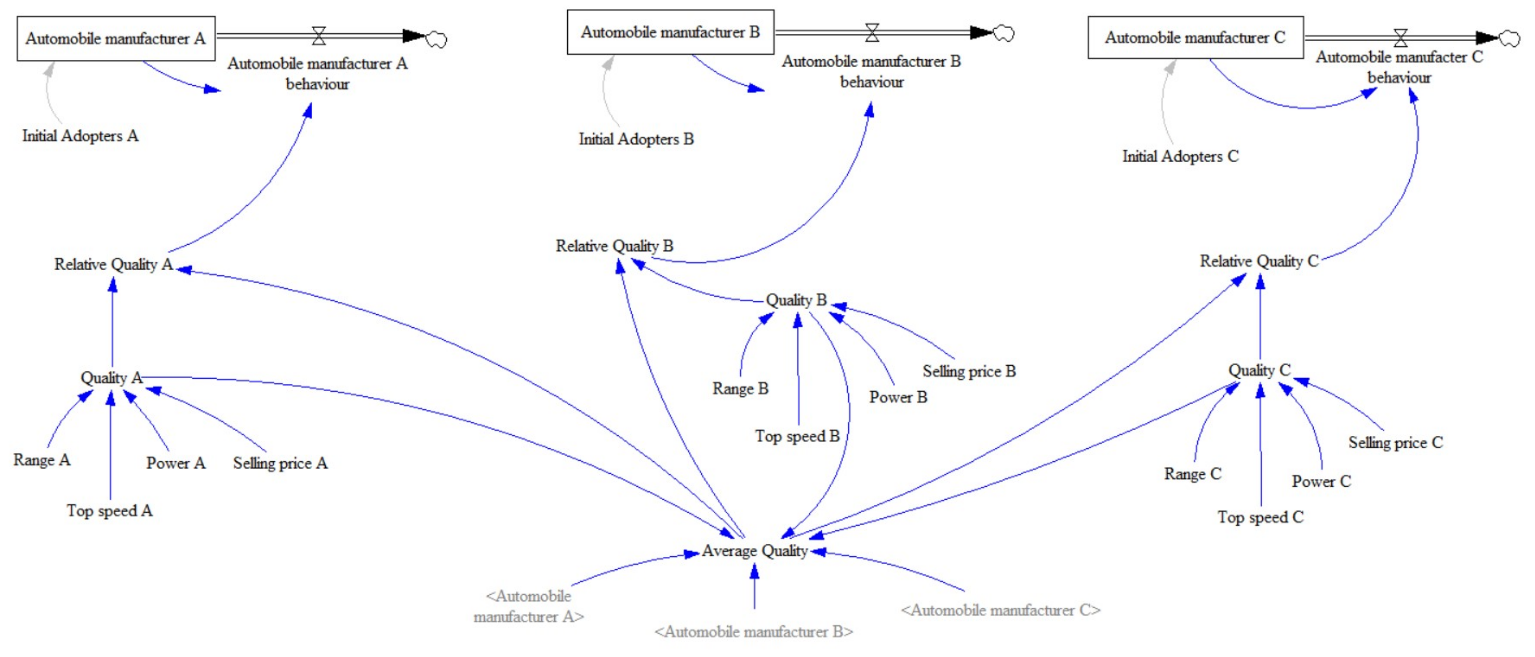
\includegraphics[width=0.9\linewidth]{img/vensim-model-pedro.png}}
\caption{Stock and Flow Diagram of Electric Vehicles adoption. Source: \cite{pedro-report}}
\label{fig:vensim-model-pedro}
\end{figure}

In this study, the author analyzed the market share evolution, average quality and relative quality of electric vehicles throughout a period of 12 months. This analysis allowed the author to conclude that, given the studied scenario, the most important decision factors would be: \textbf{price} and \textbf{charging time} and that the manufacturer with the best balance between these two factors, regardless the initial adopters, would eventually take up most of the market share of electric vehicles.

Although this study brings helpful insight to what factors could make a specific manufacturer succeed over the others, it fails to provide an understanding on how the EV market would evolve over the next years taking into consideration important factors to the consumers' choice. As I said in section \ref{section:intro}, environmental concerns are more and more present in today's society and it's helpful to better understand how the EV market will evolve to better grasp what will be the contribution of transport vehicles to the overall reduction of CO2 emissions and what are the factors that most dictate the growth of this market. 

Having that said, this work builds on the insights provided in \cite{pedro-report} and enhances it with a more global vision of the growth of the entire EV market that allows to grasp a broad perspective and have a means of comparing with the market of internal combustion vehicles.

\clearpage


\section{Adoption Factors} \label{section:factors}
As mentioned in section \ref{section:abstract}, this study is consumer-centred, which means that the study of adoption of electric vehicles is performed taking into consideration the factors that the consumer is more "passionate" about when choosing an electric vehicle. Therefore, the logic way to find these adoption factors is to base our selection on consumer-focused surveys. Particularly, the selection of factors that were chosen to this study were based on the information gathered from the surveys referenced in \cite{thesis-base, yue-xiang-paper}.

Having said that, since the model was mainly based on \cite{thesis-base}, the adoption factors included are very similar with the base model, with a few additional ones that I found to be as significant as the ones already taken into consideration. Thus, as referenced in \cite{thesis-base}, there are four technical factors that have the greatest impact on the consumer decision: \textbf{driving range}, \textbf{price}, \textbf{recharge infrastructure} and \textbf{recharging time}. In addition to these factors, we must also include the \textbf{effectiveness of advertising} such vehicles, the \textbf{word of mouth effect} and last, but not least, the \textbf{environmental concern effect}.

\subsection{Driving Range}
The maximum driving range of an EV is mostly related to the performance of the battery. Nowadays, the improvements in lithium-ion battery technology allows driving ranges on average around 200km - 300km. However, following current events, there have been some interesting developments in the field, promoted by Tesla and what currently is one of the downsides of EVs (when compared to the autonomy values of fossil fuel cars) could, in the near future, be a major advantage.

\subsection{Price}
The current purchase price of an electric vehicle is, in general, twice that of a comparable fossil fuel car (e.g. gasoline or diesel). With the mass production of more and more models, this price will eventually go down, but how fast this will happen is the difference between a more quick or slow mass adoption of EVs, which actually is kind of a paradox.

The problem with this price point is that the general consumer is not willing to pay this amount of money for an EV in contrast with governments and fleet operators that are more open to these types of purchases. However, one key factor that has been playing a big role as an incentive to the general consumer is the benefit most governments have been allowing when buying an EV, such as subsidies and/or tax reduction.

\subsubsection{Fixed Price}
The high purchase price of an EV is mostly due to the high battery prices and low production volumes. However, this premium cost for EVs is still compensated by the low cost of electricity compared to gasoline. The predictions state that, over time, the electric vehicle costs will decrease as the result of ongoing R\&D, learning effect and mass production.

\subsubsection{Variable Price}
EVs, in addition to benefiting from the lower cost of electricity when compared to fossil fuels, are also influenced by other "external" factors that do have an impact on the variable costs difference between an EV and fossil fuel vehicles, such as the rising oil prices which could make ICVs less attractive and lower maintenance costs. However, battery devaluation and the effect of environmental temperature have their own impact too, being some of the greatest disadvantages of EVs. Furthermore, there are subsidies that should stimulate the early adoption of electric vehicles.

Simplifying, the variable costs depend on a set of different values: the \textbf{influence of oil} and \textbf{electricity price}, \textbf{subsidies}, \textbf{maintenance costs}, \textbf{R\&D influences} and \textbf{devaluation of the battery}. Finally, among all these variable costs, the subsidies are the best values to influence and manipulate in simulation scenarios.

\subsection{Recharge Infrastructure}
Availability of charging infrastructure is essential to the market adoption of electric vehicles. Furthermore, the different charging alternatives, for instance the fast charging stations and the infrastructure density have a big influence on the electric vehicle's range and charging times, which additionally affects the possible market share. Which this means is that a high density of infrastructure charging locations (and fast recharge times) makes more acceptable a lower maximum driving range in comparison with a low density and slow recharge times.

\subsection{Recharging Time}
Overall, an electric vehicle requires a battery capacity of 65kWh or more to drive a 300km range. This means that it will take 5 - 6,5 hours to recharge the EV in one's garage. In the case of three phase charge station, that are more common in large homes, offices and firms, it will take approximately 1 - 1,5 hours to fully recharge the vehicle.

Besides the two types of recharging possibilities, there is also another which is mentioned as a fast charging station, despite being a lot faster, has some disadvantages because they are too expensive, making it much more difficult (almost impossible, at least right now) to include this type of research into the electric vehicle.

\subsection{Effectiveness of Advertising}
The adoption from advertisement depends on the advertising effect. This means that, depending on how effective the advertisements are, the rate of adoption will be faster or slower.

The advertising effect works in a way that the adopters made the decision on buying an EV solely on the advertising strategy (websites, pilot projects, commercials, etc.) and the major obstacle to the success of this effect is the newness of EVs that keeps potential adopters from buying one.

\subsection{Word of Mouth Effect}
The adoption by word of mouth is estimated taking into consideration Portugal's population, a contact rate and the adoption fraction that will be further explained in the next section.

This factor creates an upper limit for the adoption model and has a dissemination behaviour similar to a contagious disease, that is, the greater the number of people adopting EVs and talking about their potentially positive experience, the greater the effectiveness of the word of mouth effect. This means that in early stages of EVs market introduction this is a minor factor, but over time, becomes a much bigger influence on the market growth.

\subsection{Environmental Concern Effect}
The last factor is selected over the observation that more and more people have a very real concern about our planet and environment and being the fossil fuels industry one of biggest responsible for worldwide pollution, this factor is more and more real and is supposed to have a big impact on the EV market in the near future.

\clearpage

\section{System Dynamics Model} \label{section:model}
This chapter provide explanation and details regarding the developed model in Vensim. Before further scrutinize the implementation and for the sake of simplicity \textbf{some of the variable definitions are going to be presented as graphs}. This is because, as stated before, \textbf{this study is mostly based on the results of surveys}, hence, the best way to define some of the variables is to use the resulting data form those surveys, instead of a pure mathematical definition.

In the \textbf{cases where the variables function were define through data}, this \textbf{data was based from \cite{thesis-base, pedro-report} and adapted to the Portuguese scenario and reality using external sources}, such as news articles \cite{dv-news-article, eco-news-article, obs-news-article, uve-news-article}. Finally, to implement this types of variable functions, it was used the feature \textbf{Lookups} of Vensim, showcased in section \cite{vensim-youtube-lookups}.

\subsection{Proposed System Dynamics Model}
An can be seen in the figure \ref{fig:vensim-model}, the developed model takes into account all the factors discussed in section \ref{section:factors}.

\begin{figure}[!htbp]
\centerline{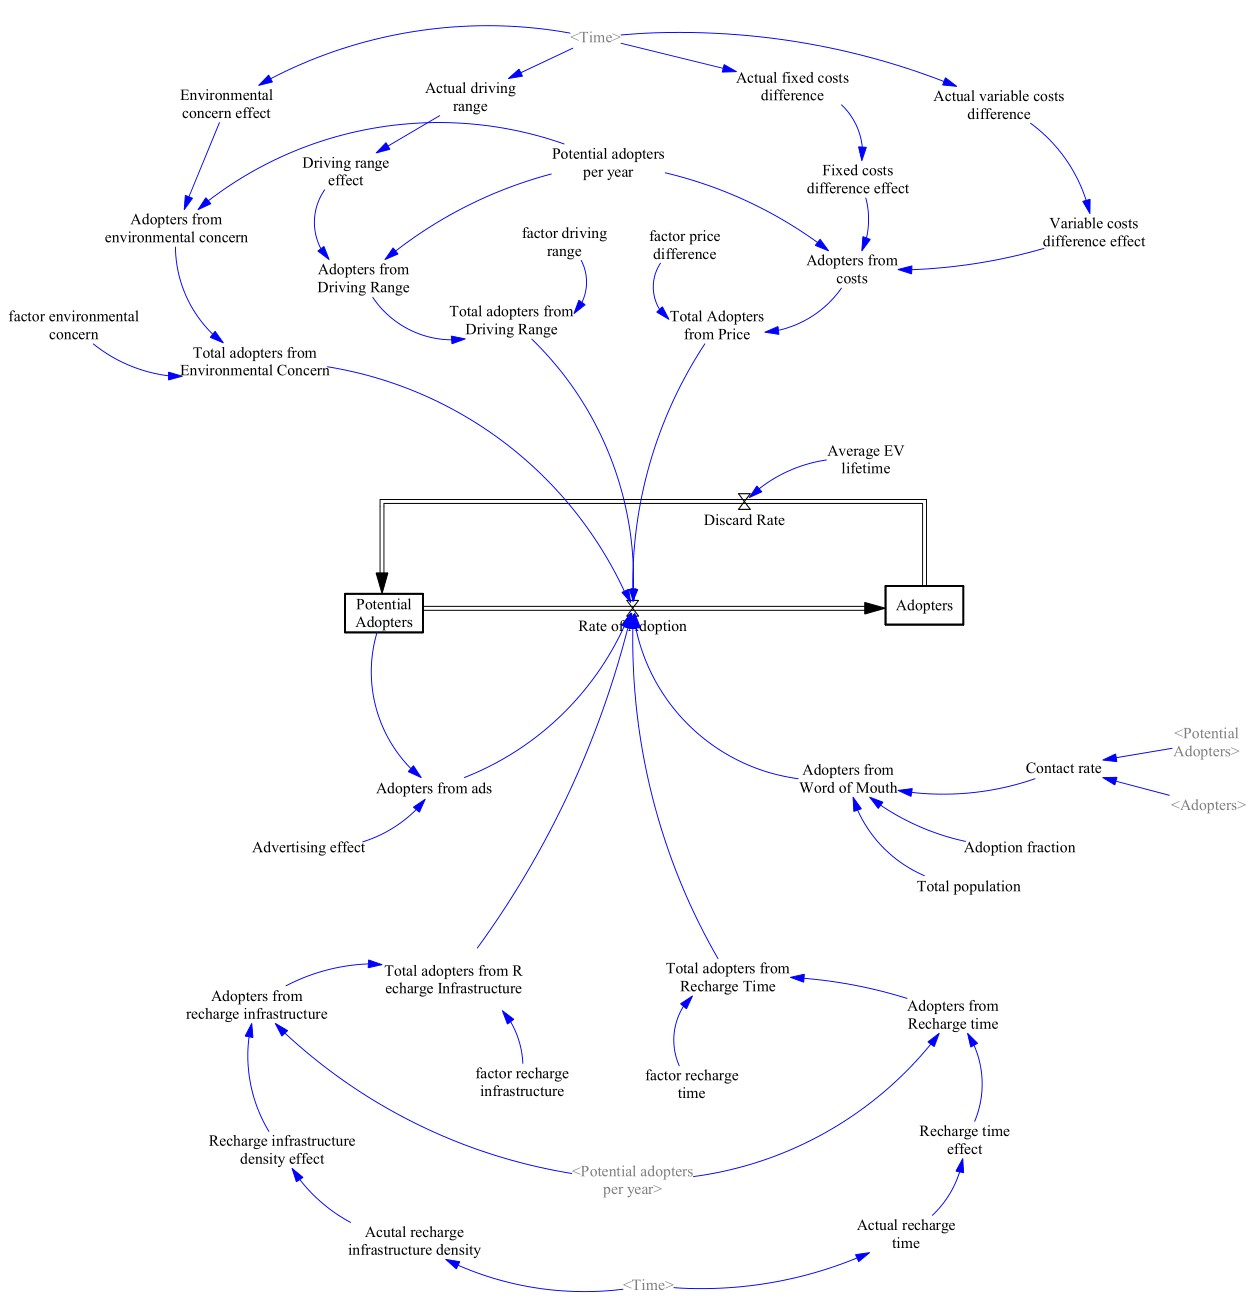
\includegraphics[width=0.74\linewidth]{img/vensim-model.jpg}}
\caption{Complete Model of EV Adoption Process}
\label{fig:vensim-model}
\end{figure}

\clearpage

Before going into detail on each factor representation and associated relationships, let's first explore the adopted layout with \textbf{Potential Adopters $\rightarrow$ Actual Adopters} and \textbf{Discard Rate}.

\subsubsection{Potential Adopters $\rightarrow$ Actual Adopters}
This model starts with the potential adopters, which are the current passenger vehicle drivers and account for approximately 6.5 million Portuguese drivers. Taking the model into consideration we can clearly see that through the rate of adoption, a fraction of these 6.5 million drivers will become adopters each ear, that is, will purchase an EV. The adopters variable has an initial value of 16 000 drivers, that represents the Portuguese drivers that already have an electric vehicle in 2020. 

\subsubsection{Discard Rate}
The bass diffusion model is frequently described as a \textit{first-purchase} model because it does not grasp the situation where the product is consumed, upgraded or discarded. What this means is that the bass diffusion model is not able to represent the inverse situation (Actual Adopters $\rightarrow$ Potential Adopters). The implemented model has the capability to capture that situation in the sense that an EV can, for instance be discarded or upgraded due to the battery lifetime or dissatisfaction. This event is modelled with the battery lifetime that has a value of 15 years. 

\subsection{Variables Definition}
The \textbf{variables} that are going to be \textbf{explored with more detail in the next sub-chapters are} the ones that were \textbf{based on data from the surveys}. It is going to be presented the graphs associated with each one of these variables and will also be explored its context beyond the number representation. All the remaining variables (that are simple mathematical functions or constants) are summarized in the table \ref{table:model-summary}, further ahead.

\subsubsection{Driving Range}
Given the current average capacity of the batteries on the market and the past years of evolution, figure \ref{fig:driving-range} describes the current average of EV's maximum range at 250km, at year 0 (2020), and an evolution to 300km after 5 years (2025), all the way to 675km at 2040. Obviously the further we predict, the less reliable are those predictions, so some of these number are, as said, just predictions and can be wrong, but are the best possible predictions given the data we have today.

Figure \ref{fig:driving-range-effect} shows us the acceptance percentages of EVs maximum range according to the consumer's responses on the surveys. The graph shows us that, even today, the average driving range it's not very well accepted, since only 5\% - 10\% of the enquired customers would buy a vehicle with that range. The minimum driving range that has a certain degree of acceptance is 440km, so it can be expected that this factor could have a big positive impact on EV sales from 2030. Obviously this is not the only factor to consider as we will see further ahead that a good recharge infrastructure with high charging speeds could lessen the need for higher driving range values.

\vspace{2cm}

\begin{figure}[htbp]
\centering
\begin{subfigure}{0.5\textwidth}
  \centering
  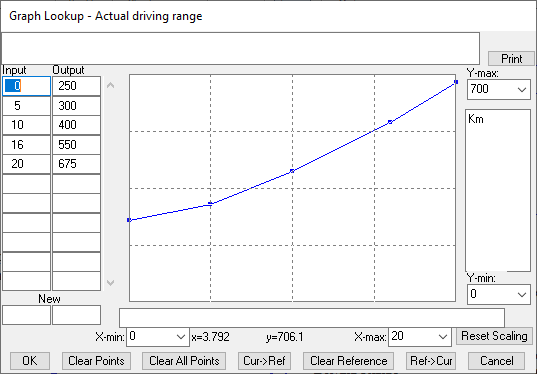
\includegraphics[width=0.98\linewidth]{img/driving-range.png}
  \caption{Actual Driving Range Data}
  \label{fig:driving-range}
\end{subfigure}%
\begin{subfigure}{0.5\textwidth}
  \centering
  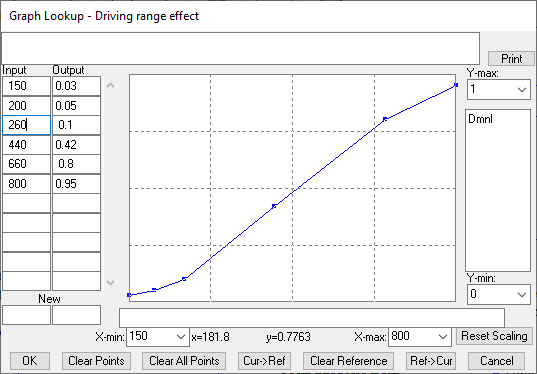
\includegraphics[width=0.98\linewidth]{img/driving-range-effect.png}
  \caption{Driving Range Effect Data}
  \label{fig:driving-range-effect}
\end{subfigure}
\caption{Driving Range Functions}
\label{fig:driving-range-funcs}
\end{figure}

\subsubsection{Price}
Considering the high costs of the lithium-ion batteries, electric vehicles tend to have a higher selling price than combustion models of the same range. Figure \ref{fig:fixed-costs} shows us precisely that. At 2020, 0-year, the average price difference between an EV and an ICV is 10 000\euro, which means that, an electric vehicle costs 10 000\euro \space more than a similar ICV model. After 5 years, this difference is around 5000\euro, that is, in 5 years the difference of prices has reduced over 50\%. At 2040 the price difference is in all-time low of 1900\euro, reducing the price difference to 20\% of its initial value.

\begin{figure}[htbp]
\centering
\begin{subfigure}{0.5\textwidth}
  \centering
  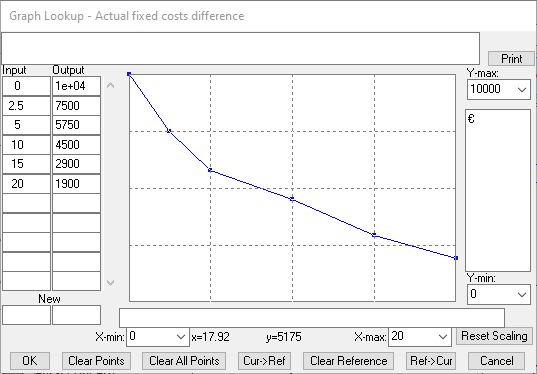
\includegraphics[width=0.98\linewidth]{img/fixed-costs-difference.png}
  \caption{Actual Fixed Costs Difference Data}
  \label{fig:fixed-costs}
\end{subfigure}%
\begin{subfigure}{0.5\textwidth}
  \centering
  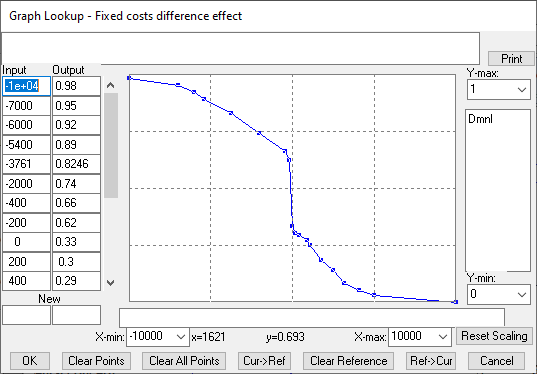
\includegraphics[width=0.98\linewidth]{img/fixed-costs-difference-effect.png}
  \caption{Fixed Costs Difference Effect Data}
  \label{fig:fixed-costs-effect}
\end{subfigure}
\caption{Fixed Costs Difference Functions}
\label{fig:fixed-costs-funcs}
\end{figure}

Figure \ref{fig:fixed-costs-effect} shows us the acceptance percentages of these differences in price regarding EV and ICV models. From the graph, we can understand that the majority of people can only consider purchase an EV when its price is the same or less than an equivalent ICV. If we would only consider this factor, we would wrongly think that, even 20 years from now, only a minority of the population would buy an EV. The aspect that we must have in consideration is the variable costs such as oil pricing, government subsidies and/or tax the reduction, electricity price. Some of these factors significantly amortize the price difference, either instantly or over time.

\subsubsection{Recharge Infrastructure}
As said before, the recharge infrastructure is the network of recharging stations (public or private, that is, home recharge "stations" are considered as private stations) scattered all over the country and it is one of the most important differences between the EV and ICV markets. As figure \ref{fig:recharge-infra} clearly demonstrates, today we have an average density of 100km between each station and this value is actually deceitful, because it does not represent evenly all Portuguese territory. The predictions suggest that in 20 years, Portugal will have an average density of recharge stations around 0km - 5km, which is actually very optimistic.

\begin{figure}[htbp]
\centering
\begin{subfigure}{0.5\textwidth}
  \centering
  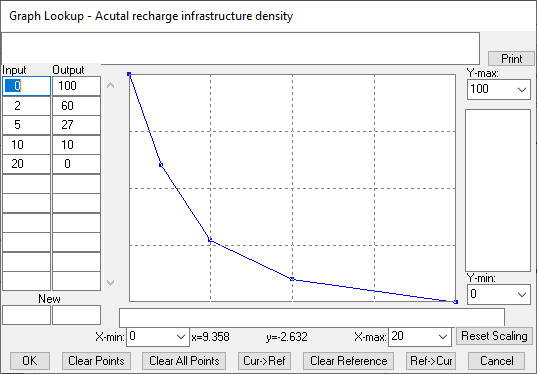
\includegraphics[width=0.98\linewidth]{img/recharge-infra-density.png}
  \caption{Actual Recharge Infrastructure Density Data}
  \label{fig:recharge-infra}
\end{subfigure}%
\begin{subfigure}{0.5\textwidth}
  \centering
  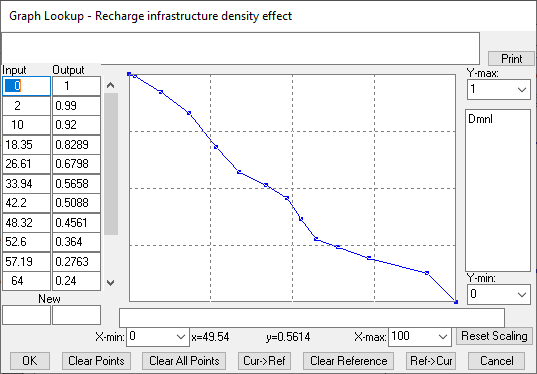
\includegraphics[width=0.98\linewidth]{img/recharge-infra-density-effect.png}
  \caption{Recharge Infrastructure Density Effect Data}
  \label{fig:recharge-infra-effect}
\end{subfigure}
\caption{Recharge Infrastructure Density Functions}
\label{fig:recharge-infra-funcs}
\end{figure}

Figure \ref{fig:recharge-infra-effect} allows us to better understand what the consumer thinks of this factor. According the surveys, the great majority of the population believes that the acceptable recharge infrastructure density is between 0km and 40km.

\subsubsection{Recharging Time}
If we own an ICV and we are close to run out of fuel, the process of refuel our vehicle could not be simpler or faster, taking no more than 5 minutes to fill the tank. In the case of electric vehicles the currently reality is not quite the same, since, currently, the action of completely recharging a EV can take up to 6,5 hours. Figure \ref{fig:recharge-time}, show us that 5 years from now, the process of recharge an EV could be less time consuming, taking at most 5 hours to fully charge an EV and that 20 years from now the same process will be significantly faster taking 2 minutes to be completed, thanks to the switch of a discharged battery (that will be promptly recharged) for a fully charged one.

In figure \ref{fig:recharge-time-effect} we can see that more than 40\% of the enquired population considers that the acceptable time to fully recharge an EV battery (or switch it with a recharged one) should be less than 50 minutes.

\vspace{1cm}

\begin{figure}[htbp]
\centering
\begin{subfigure}{0.5\textwidth}
  \centering
  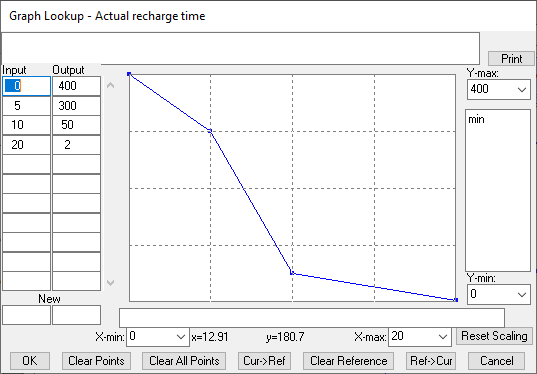
\includegraphics[width=0.89\linewidth]{img/recharge-time.png}
  \caption{Actual Recharge Time Data}
  \label{fig:recharge-time}
\end{subfigure}%
\begin{subfigure}{0.5\textwidth}
  \centering
  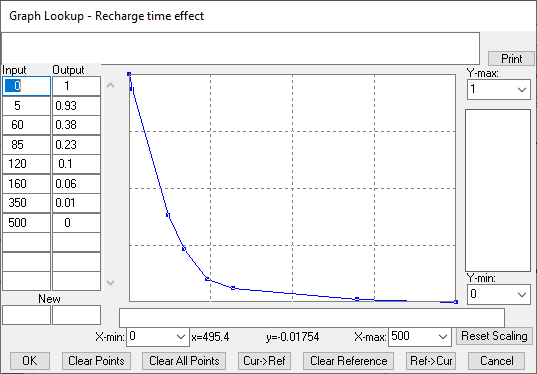
\includegraphics[width=0.89\linewidth]{img/recharge-time-effect.png}
  \caption{Recharge Time Effect Data}
  \label{fig:recharge-time-effect}
\end{subfigure}
\caption{Recharge Time Functions}
\label{fig:recharge-time-funcs}
\end{figure}

\subsubsection{Environmental Concern Effect}
More and more people are concerned with the future of our planet, so, this concern has an impact on EV sales. As can be seen in figure \ref{fig:env-concern}, at early stages this concern has a boost effect on sales around 5\%, this value starts to increase at fast pace in the next 12,5 years and then, as EVs become more and more common, its growth starts to slow down due to the loss of the novelty effect and the loss of the big disruption impact on people's lives and pollution percentages.

\begin{figure}[htbp]
\centerline{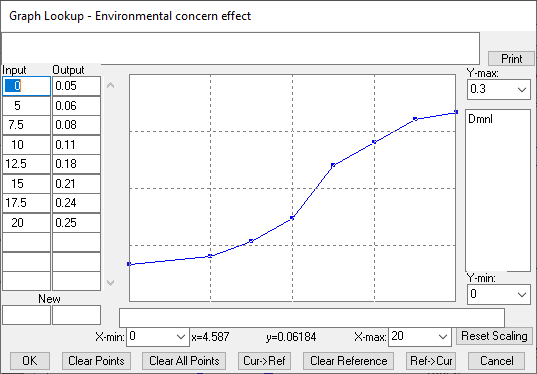
\includegraphics[width=0.45\linewidth]{img/env-concern-effect.png}}
\caption{Environmental Concern Effect}
\label{fig:env-concern}
\end{figure}

\subsection{Weight of Factors}
This section shows how each factor influence is weighed on the implemented model. Table \ref{table:factors-weights} summarizes how the weight is distributed among all the factors.

\begin{table}[htbp]
\centering
\begin{adjustbox}{width=0.8\textwidth}
\begin{tabular}{ccccccc}
\cline{2-6}
\multicolumn{1}{l|}{} & \multicolumn{1}{l|}{\textbf{Driving Range}} & \multicolumn{1}{l|}{\textbf{Charging Time}} & \multicolumn{1}{l|}{\textbf{Price Difference}} & \multicolumn{1}{l|}{\textbf{Recharge Infrastructure}} & \multicolumn{1}{l|}{\textbf{Environmental Concern}} \\ \cline{1-6}
\multicolumn{1}{|l|}{\textbf{Weight}} & \multicolumn{1}{c|}{0.3} & \multicolumn{1}{c|}{0.06} & \multicolumn{1}{c|}{0.56} & \multicolumn{1}{c|}{0.04} & \multicolumn{1}{c|}{0.04} \\ \cline{1-6}
\end{tabular}
\end{adjustbox}
\caption{Weight of Factors in Vensim Model}
\label{table:factors-weights}
\end{table}

\subsection{Summary of Model Variables}
Table \ref{fig:vensim-model} summarizes the entire model, listing all variables with its equations/initial values and units.

\begin{table}[!htpb]
   \centering
   \begin{adjustbox}{width=0.96\textwidth}
   \begin{tabular}{|l|l|l|}
   \hline
   \textbf{Variable} & \textbf{Equation/ Initial Value} & \textbf{Units} \\\hline
   INITIAL TIME & \textit{0} & \textit{Year} \\\hline
   FINAL TIME & \textit{20} & \textit{Year} \\\hline
   Potential Adopters & \makecell[l]{\textit{INTEG(Discard Rate - Rate of Adoption, \num{6.5e+6})}} & \textit{Person} \\\hline
   Rate of Adoption & \makecell[l]{\textit{Total adopters from Driving Range + Adopters from ads + Total Adopters from Price + } \\ \textit{Total adopters from Recharge Infrastructure + Total adopters from Recharge Time +} \\ \textit{ + Total adopters from Environmental Concern + Adopters from Word of Mouth}} & \textit{Person} \\\hline
   Adopters & \textit{INTEG(Rate of Adoption - Discard Rate, 16 000)} & \textit{Person} \\\hline
   Average EV lifetime & \textit{15} & \textit{Year} \\\hline
   Discard Rate & \textit{ 0.003 * ( Rate of Adoption / Average EV lifetime)} & \textit{Person} \\\hline
   Potential adopters per year & \textit{200 000} & \textit{Person/Year} \\\hline
   Environmental concern effect & \makecell[l]{\textit{WITH LOOKUP (Time,} \\
   \textit{([(0,0)-(20,0.3)],(0,0.05),(5,0.06),(7.5,0.08),(10,0.11),(12.5,0.18),(15,0.21),(17.5,0.24),(20,0.25) ))}} & \\\hline
   Adopters from environmental concern & \textit{Environmental concern effect * Potential adopters per year} & \textit{Person} \\\hline
   factor environmental concern & \textit{0.04} & \\\hline
   Total adopters from Environmental Concern &  \textit{factor environmental concern * Adopters from environmental concern} & \textit{Person} \\\hline
   Actual driving range & \makecell[l]{\textit{WITH LOOKUP (Time,} \\
   \textit{([(0,0)-(20,700)],(0,250),(5,300),(10,400),(16,550),(20,675) ))}} & Km \\\hline
   Driving range effect & \makecell[l]{\textit{WITH LOOKUP (Actual driving range,} \\ \textit{([(150,0)-(800,1)],(150,0.03),(200,0.05),(260,0.1),(440,0.42),(660,0.8),(800,0.95) ))}} & \\\hline
   Adopters from Driving Range & \textit{Driving range effect * Potential adopters per year} & \textit{Person} \\\hline
   factor driving range & \textit{0.3} & \\\hline
   Total adopters from Driving Range & \textit{factor driving range * Adopters from Driving Range} & \textit{Person} \\\hline
   Actual fixed costs difference & \makecell[l]{\textit{WITH LOOKUP (Time,} \\ \textit{([(0,0)-(20,10000)],(0,10000),(2.5,7500),(5,5750),(10,4500),(15,2900),(20,1900) ))}} & \textit{\euro} \\\hline
   Fixed costs difference effect & \makecell[l]{\textit{WITH LOOKUP (Actual fixed costs difference,} \\ \textit{([(-10000,0)-(10000,1)],(-10000,0.98),(-7000,0.95),(-6000,0.92),(-5400,0.89),(-3761} \\ \textit{,0.8246),(-2000,0.74),(-400,0.66),(-200,0.62),(0,0.33),(200,0.3),(400,0.29),(900,0.27} \\ \textit{),(1100,0.25),(1800,0.18),(2500,0.14),(3200,0.08),(4100,0.05),(5000,0.03),(10000,0) ))}} & \\\hline
   Actual variable costs difference & \makecell[l]{\textit{WITH LOOKUP (Time,} \\ \textit{([(0,-1000)-(20,1000)],(0,912),(13,0),(20,-707) ))}} & \textit{\euro} \\\hline
   Variable costs difference effect & \makecell[l]{\textit{WITH LOOKUP (Actual variable costs difference,} \\ \textit{([(-5000,0)-(5000,1)],(-5000,1),(-3000,0.93),(-800,0.63),(100,0.12),(400,0.07),(2100,0.01),(5000,0) ))}} & \\\hline
   Adopters from costs & \textit{(Fixed costs difference effect + Variable costs difference effect) * Potential adopters per year} & \textit{Person} \\\hline
   factor price difference & \textit{0.56} & \\\hline
   Total adopters from Price & \textit{factor price difference * Adopters from costs} & \textit{Person} \\\hline
   Advertising effect & \textit{0.00025} & \\\hline
   Adopters from ads & \textit{Advertising effect * Potential Adopters} & \textit{Person} \\\hline
   Actual recharge infrastructure density & \makecell[l]{\textit{WITH LOOKUP (Time,} \\ \textit{([(0,0)-(20,100)],(0,100),(2,60),(5,27),(10,10),(20,0) ))}} & \\\hline
   Recharge infrastructure density effect & \makecell[l]{\textit{WITH LOOKUP (Actual recharge infrastructure density,} \\ \textit{([(0,0)-(100,1)],(0,1),(2,0.99),(10,0.92),(18.35,0.8289),(26.61,0.6798),(33.94,0.5658),(42.2,0.5088)} \\ \textit{,(48.32,0.4561),(52.6,0.364),(57.19,0.2763),(64,0.24),(73.5,0.19),(91.3,0.125),(100,0) ))}} & \\\hline
   Adopters from recharge infrastructure & \textit{Recharge infrastructure density effect * Potential adopters per year} & \textit{Person} \\\hline
   factor recharge infrastructure & \textit{0.04} & \\\hline
   Total adopters from Recharge Infrastructure & \textit{factor recharge infrastructure * Adopters from recharge infrastructure} & \textit{Person} \\\hline
   Contact rate & \textit{Potential Adopters / Adopters} & \\\hline
   Adoption fraction & \textit{0.01} & \\\hline
   Total population & \textit{\num{1.028e+07}} & \textit{Person} \\\hline
   Adopters from Word of Mouth & \textit{Total population / Contact rate * Adoption fraction} & \textit{Person} \\\hline
   Actual driving range & \makecell[l]{\textit{WITH LOOKUP (Time,} \\
   \textit{([(0,0)-(20,400)],(0,400),(5,300),(10,50),(20,2) ))}} & min \\\hline
   Recharge time effect & \makecell[l]{\textit{WITH LOOKUP (Actual recharge time,} \\ \textit{([(0,0)-(500,1)],(0,1),(5,0.93),(60,0.38),(85,0.23),(120,0.1),(160,0.06),(350,0.01),(500,0) ))}} & \\\hline
   Adopters from Recharge time & \textit{Recharge time effect * Potential adopters per year} & \textit{Person} \\\hline
   factor recharge time & \textit{0.06} & \\\hline
   Total adopters from Recharge Time & \textit{factor recharge time * Adopters from Recharge time} & \textit{Person} \\\hline
   \end{tabular}
   \end{adjustbox}
   \caption{Model Summary | variables and functions}
   \label{table:model-summary}
\end{table}

\clearpage

\section{Results and Discussion} \label{section:results}
In this chapter are presented some scenarios and tests with extreme value changes to better understand how the market could evolve in the near future and is also very useful to detect flaws in the model.

\subsection{Basic scenario}
The basic scenario is based on the values explained throughout section \ref{section:model}. Figure \ref{fig:adopters} shows an exponential growth of the population of adopters, characterized by a slow
but steady growth in the beginning (year 2020-2027), and a large growth in the end (year 2028-
2040). In figure \ref{fig:adoption-rate} can also be seen the adoption rate with an exponential behavior, especially in the first 15 years. Both results are obviously connected, by the model definition, and this exponential growth is due to the fact that, as seen earlier, most of the factors are in the acceptable conditions "imposed" by the customers after the first 10 years, meaning that after those 10 years (in 2030) the consumers start more easily and frequently purchasing electric vehicles, hence, the exponential growth.

\begin{figure}[htbp]
\centering
\begin{subfigure}{0.55\textwidth}
  \centering
  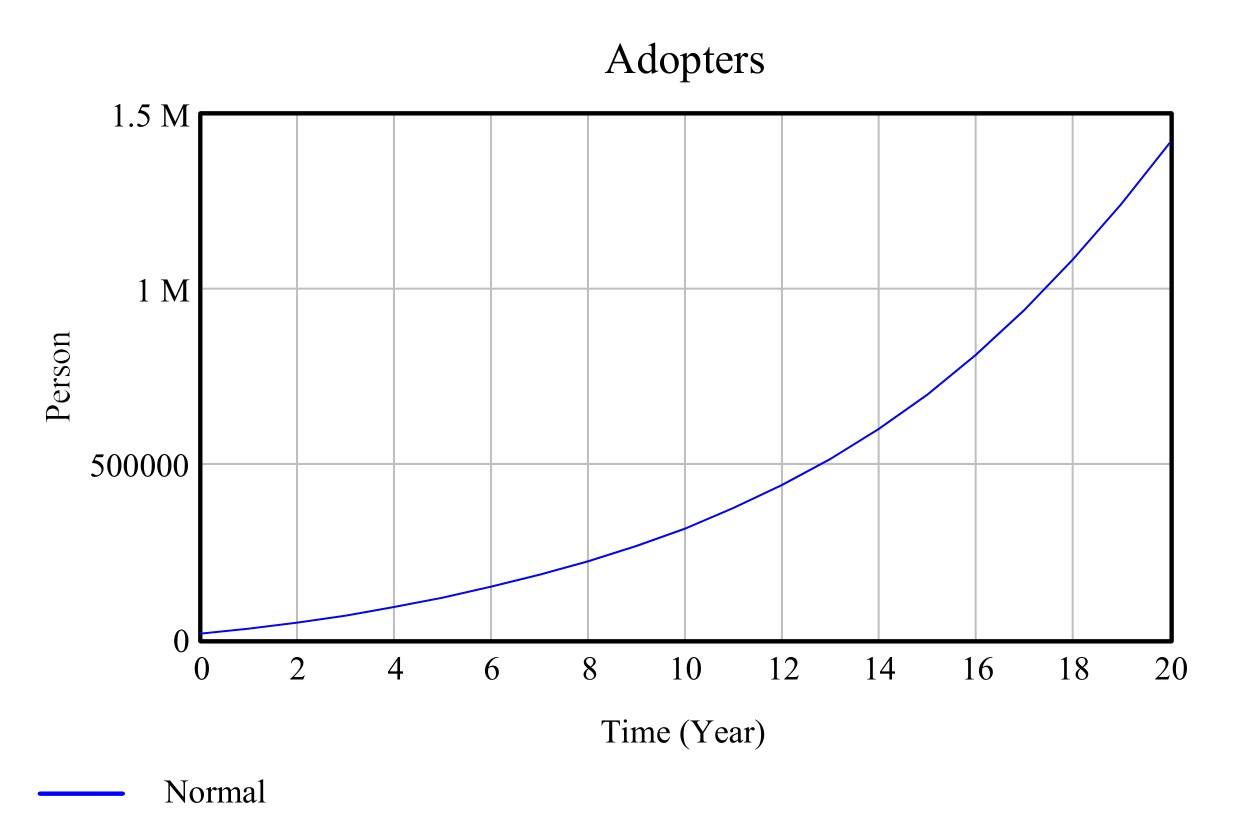
\includegraphics[width=0.98\linewidth]{img/results-basic.jpg}
  \caption{Adopters growth/evolution over the years}
  \label{fig:adopters}
\end{subfigure}%
\begin{subfigure}{0.45\textwidth}
  \centering
  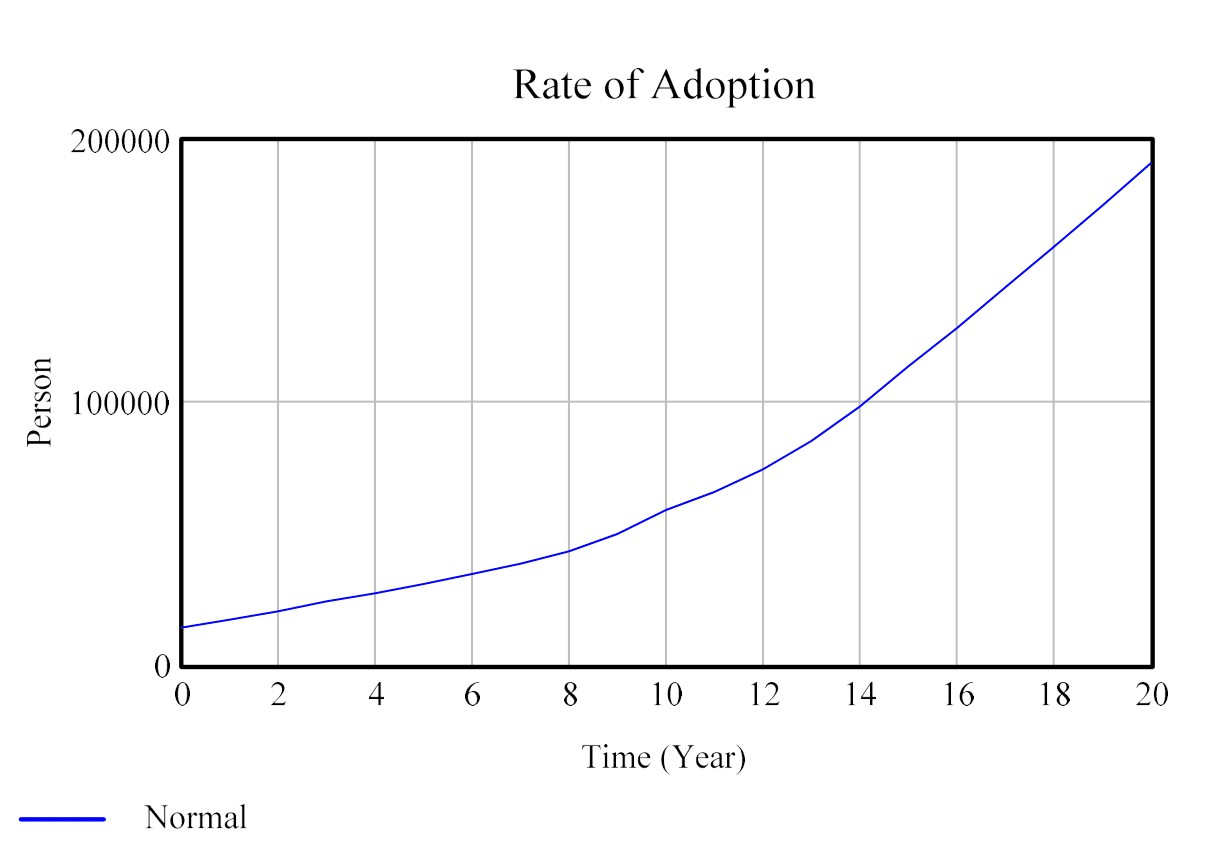
\includegraphics[width=0.98\linewidth]{img/results-basic-adoption-rate.jpg}
  \caption{Rate of Adoption over the years}
  \label{fig:adoption-rate}
\end{subfigure}
\caption{Graphical representation of basic scenario results}
\label{fig:basic-scenario}
\end{figure}

\subsection{Scenario Situations}
Scenario situations use the same values for the model as in the basic situation except from the variable that is being tested or changed to simulate a particular scenario and are useful to create insights for the model and to make the assumptions more reliable.

\subsubsection{Price Difference Effect}
The price difference between an EV and an ICV is the most crucial factor that keeps potential adopters from purchasing an EV. According to the surveys and the information portrayed in section \ref{section:model}, the area around a zero (or negative) price difference has the most effect on the adopters. In contrast to others factors such as driving range, the price difference can be "artificially" influenced through subsidies given by the government. Therefore the subsidy scenario is given in a situation where the government would provide a subsidy of 5000\euro \space on the vehicle fixed price from 2020 to 2029, that is, the first 9 years.

\begin{figure}[htbp]
\centerline{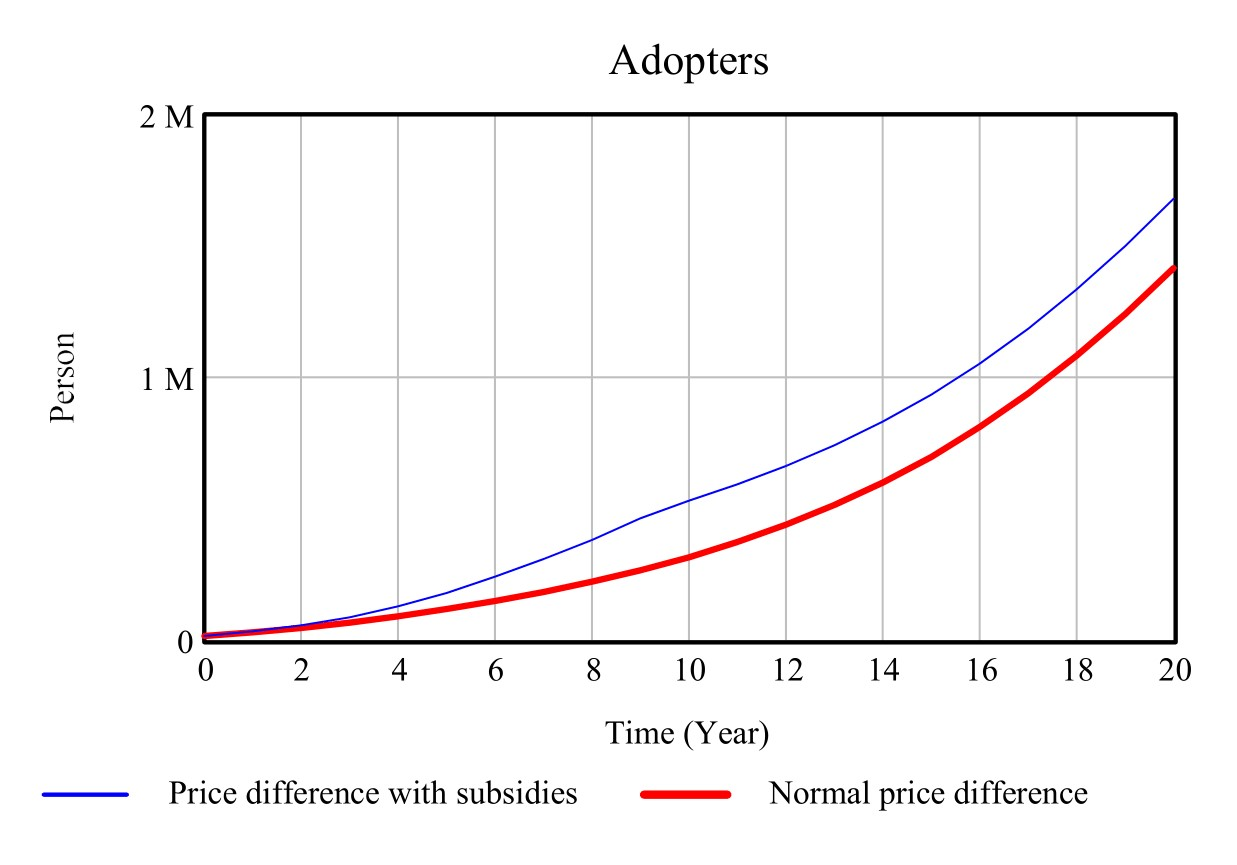
\includegraphics[width=0.7\linewidth]{img/results-price-difference.jpg}}
\caption{Adopters Growth in function of Price Difference variations}
\label{fig:results-price-difference}
\end{figure}

Figure \ref{fig:results-price-difference} shows the result of the scenario described above. As we can see in the graph, the subsidy allowance was effective in the sense that in the first 9 years, the adoption rate clearly increased because in the same time-frame the scenario with the subsidies had a bigger growth of adopters than the basic one. After those 9 years, the adoption rate decreases a little and approximates to the adoption rate of the basic scenario. This "boost" on the first 9 years was able to positively influence the EV market as we ended the 20-year time-frame with considerably more EV adopters in the altered scenario when compared to the basic one. 

\subsubsection{Infrastructure Network Density and Recharge Time Effect}
In this section, the study focuses on the infrastructure network density and the recharge time effects on the EV market.

In this verification, there are 3 different scenarios: \textbf{the normal one}, \textbf{the scenario with a high density infrastructure and slow charging times} and one last \textbf{scenario with a high density infrastructure and fast charging capabilities}. The normal one is the basic scenario referenced earlier.

The other two scenarios have a high density recharging network, meaning that we have total coverage on Portuguese territory from the start (year 2020). The graph of the actual recharge network density in these scenarios has a similar appearance/behaviour to the normal one, being the only difference the starting value that in these scenario has a value of density of 10km, instead of 100km.

What sets these two scenarios apart is the charging times, in one of them, we have slow charging capabilities (with a initial value of 8 hours) and in the other we have fast charging capabilities (with a initial value of 30 minutes).

The time range is set to 10 years, because this better shows the effect of the infrastructure and recharging times in the early phase of the adoption process.

\begin{figure}[htbp]
\centerline{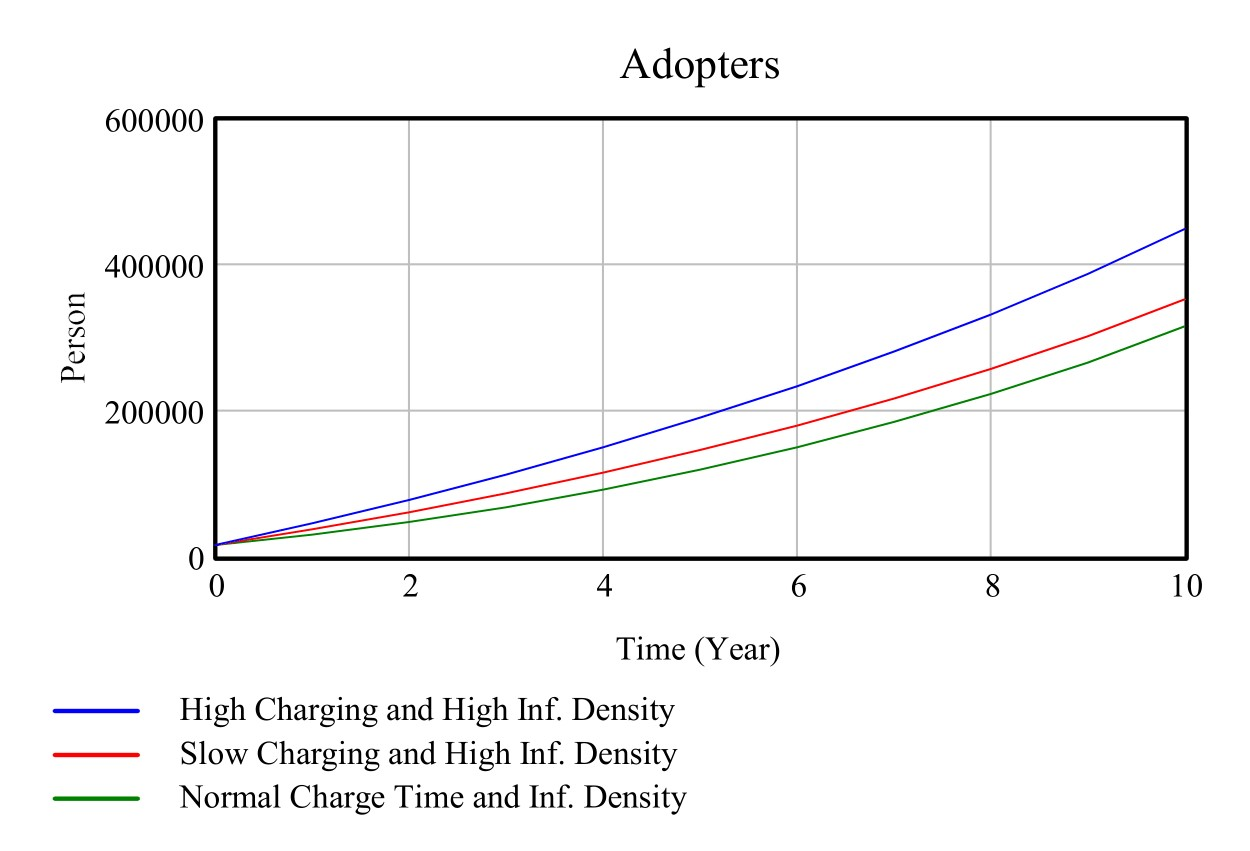
\includegraphics[width=0.7\linewidth]{img/results-time-and-density.jpg}}
\caption{Adopters Growth in function of Infrastructure Density and Charging Time variations}
\label{fig:results-time-and-density}
\end{figure}

Figure \ref{fig:results-time-and-density} shows the result of the scenario described above. As we can see in the graph, these scenario simulations allows us to conclude that the population of adopters increases as result of both \textbf{high infrastructure density} and \textbf{fast charging capabilities}. As we can see, the scenario with high recharge infrastructure density and slow charging is still able to "produce" more adopters than the basic scenario. This is related with the premised stated earlier that a high density recharge network allows for slower charging times, because there is high availability of charging stations. The optimal scenario is when we have a high density charging infrastructure and fast charging capabilities from the start, being these two conditions the best of both worlds. However, a optimistic yet feasible scenario is to have a high density charging network in the early stages of EV introduction (first 10-15 years) and then focusing on improve the charging times of the already existent EV charging stations.

\clearpage

\section{Conclusions}
From what was possible to understand from this study, it can be concluded that when we are dealing with a market research study, consumers' input and opinion is crucial to accurately grasp and understand the importance of multiple factors and their relationships in the respective market.

Furthermore, considering the model described in section \ref{section:model} and its respective results, detailed in section \ref{section:results}, it is clear that, despite the current limited capabilities of the underlying technology and the restricted technological evolution of Electric Vehicles, the growth of the EV market, regarding its population of adopters has an exponential behaviour, leading to the belief that, at some point in the future, the personal vehicles market will be dominated by EVs.

Moreover, it also reasonable to conclude that a major factor to help accelerate the purchase of EVs and promote its further development is the government subsidies, being the price one of the greatest obstacles to consumers when considering to buy an EV. The other obstacle to current EV adoption is the driving range of these vehicles, that is quite limited in current models, however, the implementation of a well distributed recharging infrastructure with optimal coverage is key to minimize this factor and mitigate the existent doubt of transportation viability with an EV.

\clearpage

\bibliography{refs}
\bibliographystyle{ieeetr}

\end{document}
